\documentclass[11pt,fontset=fandol]{ctexart}
\usepackage[a4paper,margin=1in]{geometry}
\usepackage{amsmath,amssymb,amsfonts}
\usepackage{booktabs}
\usepackage{graphicx}
\usepackage{caption}
\usepackage{enumitem}
\usepackage[hidelinks]{hyperref}
\usepackage{xurl}
\usepackage{microtype}
\usepackage{array}
\usepackage[table]{xcolor}

\title{二维单 Target 半透膜渐进扫描与出走时序机制报告\\\large Symmetric Membrane Continuation, Corridor Exit Timing, and Membrane Exit Timing}
\author{}
\date{}

\setlist{nosep}
\setlength{\textfloatsep}{8pt plus 2pt minus 2pt}
\setlength{\floatsep}{6pt plus 2pt minus 2pt}
\setlength{\intextsep}{6pt plus 2pt minus 2pt}
\setlength{\abovecaptionskip}{4pt}
\setlength{\belowcaptionskip}{0pt}
\setlength{\tabcolsep}{5pt}
\renewcommand{\arraystretch}{1.10}

\begin{document}
\maketitle

\section*{结论先行}
这份 companion report 只做一件事：在固定对称 one-target soft-corridor baseline 的前提下，把 ``什么时候走出 corridor'' 与 ``什么时候真的穿膜'' 这两件事分开。

主结论有四条：
\begin{enumerate}
  \item 从 \(\kappa=0\) 到 \(\kappa=0.006\) 的对称膜渐进扫描里，双峰并没有被膜新建出来；它在 fully reflective control 下已经存在，而且整个 continuation 上始终保持 \texttt{phase=1}。
  \item `fully reflective` 情况下，\(\tau_{\mathrm{mem}}\equiv\infty\)，但 \(\tau_{\mathrm{out}}\) 仍然可以非零，因为左端开口允许 walker 从 corridor 绕到外侧。
  \item later windows 的 slow branch 主要对应 ``先离开主 corridor，再较晚返回并命中''，而不是 ``先到 target funnel 再被卡住''。
  \item 膜穿越会增强 later windows；继续把 \(\kappa\) 推到临界带后，`peak2` 的 membrane-assisted mass 会在 \(\kappa\approx 0.014\) 左右超过 \(50\%\)，但这种 ``接管'' 只发生在双峰塌缩前夕：\(\texttt{phase}=1\) 只维持到 \(\kappa=0.0152\)，而 \(\kappa=0.0153\) 即跌成 \(\texttt{phase}=0\)。
\end{enumerate}

\section{基线与两个 timing observable}
本稿固定的几何与驱动是
\[
L_x=60,\qquad W_y=15,\qquad (x_s,y_s)=(7,7),\qquad (x_t,y_t)=(58,7),
\]
corridor band 为 \(y=5,\dots,9\)，膜 span 为 \(x=5,\dots,54\)。局部右推只作用在主通道段 \(5\le x\le 54,\ 5\le y\le 9\)，强度取
\[
\delta_{\mathrm{core}}=0.8,\qquad \delta_{\mathrm{open}}=0.0,
\]
同时全空间仍叠加一个较弱的全局左向偏置 \((b_x,0)=(-0.08,0)\)。本报告只扫描对称通透率
\[
\kappa_{c\to o}=\kappa_{o\to c}=\kappa\in\{0,0.00025,\dots,0.0060\},
\]
并对每个 \(\kappa\) 用统一长时 horizon \(t_{\max}=40000\) 重算 exact \(f(t)\)、双峰窗口和 timing observable。
此外，为了回答 ``膜相关路径会不会最终接管第二峰''，本稿还单独做了一段临界带 probe：
\[
\kappa\in\{0.0120,0.0130,0.0140,0.0145,0.0148,0.0149,0.0150,0.0151,0.0152,0.0153\}.
\]

我们关心的两个 first-event time 是：
\[
\tau_{\mathrm{out}}=\inf\{t\ge 1: X_t\notin C\},
\qquad
\tau_{\mathrm{mem}}=\inf\{t\ge 1:(X_{t-1},X_t)\in E_{\mathrm{mem}}^{c\to o}\},
\]
其中 \(C\) 是 corridor band，\(E_{\mathrm{mem}}^{c\to o}\) 是 corridor-to-outside 的定向膜边。前者记录 ``第一次离开 corridor''，后者只记录 ``第一次真的穿膜''。因此：
\begin{itemize}
  \item \(\tau_{\mathrm{out}}\) 在 \(\kappa=0\) 时仍然可能发生；
  \item \(\tau_{\mathrm{mem}}\) 在 \(\kappa=0\) 时必须严格为零事件。
\end{itemize}

窗口仍按 repo-native rule 从每个 \(\kappa\) 自己的 smoothed \(f(t)\) 上提取 \(t_{\mathrm{peak1}}, t_{\mathrm{valley}}, t_{\mathrm{peak2}}\) 与公共半宽。为了让代表图直接对准机制阈值，本文后续统一使用三组代表值：
\[
\kappa=0,\qquad \kappa=0.0140\ \text{(takeover onset)},\qquad \kappa=0.0152\ \text{(last phase-1)}.
\]
这三点上晚峰位置依次为 \(2359, 2028, 1968\)，而 \(\mathrm{sep}_{\mathrm{peaks}}\) 则从 \(0.447\) 下降到 \(0.289\) 再到 \(0.273\)。

\begin{figure}[!htbp]
  \centering
  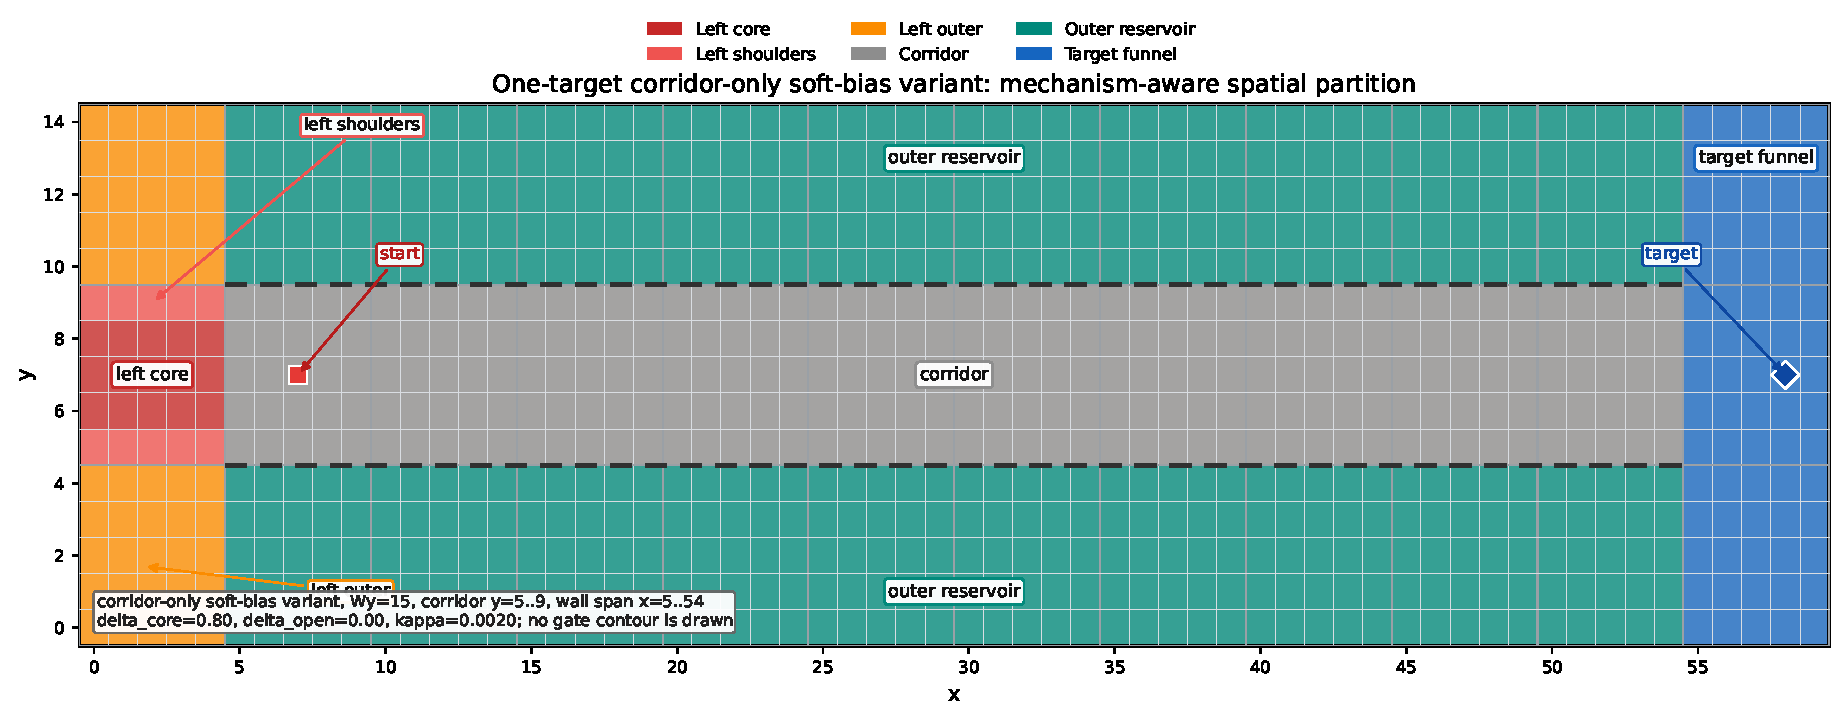
\includegraphics[width=0.82\linewidth]{../artifacts/figures/one_target_partition.pdf}
  \caption{本 companion report 复用的对称单 target 区域划分。这里主要需要记住三类空间：左侧区域、corridor band，以及 corridor 外侧的 outside reservoir。后文中 ``leaving the corridor'' 指的就是第一次从 corridor band 进入这些 outside 状态。}
  \label{fig:partition}
\end{figure}

\section{对称膜渐进扫描}
\begin{figure}[!htbp]
  \centering
  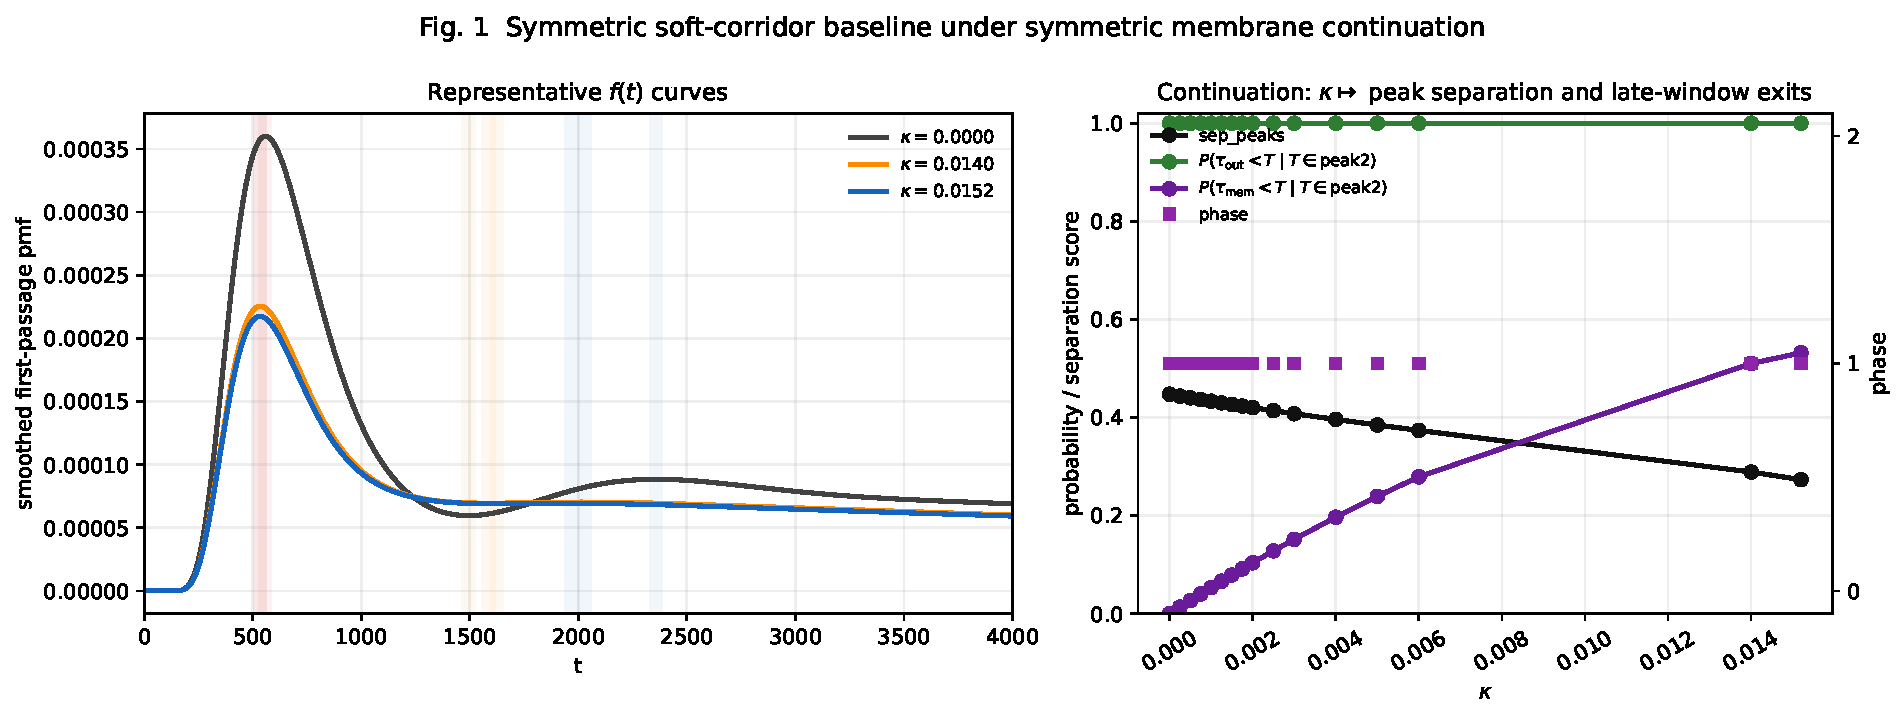
\includegraphics[width=0.98\linewidth]{../artifacts/figures/fig1_kappa_continuation.pdf}
  \caption{对称膜通透率 continuation。左图改成三条机制代表曲线：\(\kappa=0\)（baseline）、\(\kappa=0.0140\)（membrane takeover onset）与 \(\kappa=0.0152\)（最后一个 `phase=1`）。右图把基线 continuation 与这两个 critical representatives 压缩成四个量：\(\mathrm{sep}_{\mathrm{peaks}}(\kappa)\)、phase\((\kappa)\)、\(P(\tau_{\mathrm{out}}<T\mid T\in\texttt{peak2})\) 与 \(P(\tau_{\mathrm{mem}}<T\mid T\in\texttt{peak2})\)。}
  \label{fig:kappa-cont}
\end{figure}

图~\ref{fig:kappa-cont} 说明了三件事。

第一，当前 soft-corridor baseline 在整个 continuation 上都保持双峰但不属于 clear double peak：phase 始终为 \(1\)，没有随着 \(\kappa\) 升高而跳相。

第二，\(\mathrm{sep}_{\mathrm{peaks}}\) 随 \(\kappa\) 持续下降，这意味着在这组参数下，膜通透并不是把双峰 ``制造出来'' 的主因，反而在逐步压缩峰间分离；从 baseline 的约 \(0.447\) 到最后一个 `phase=1` 已降到约 \(0.273\)。

第三，\(\tau_{\mathrm{out}}\) 对 `peak2` 的条件概率几乎从一开始就接近 \(1\)，而 \(\tau_{\mathrm{mem}}\) 则从 \(0\) 增长到 takeover onset 的约 \(51.0\%\)，并在最后一个 `phase=1` 处达到约 \(53.2\%\)。所以膜相关子族最终确实会成为第二峰多数；但这个接管只发生在双峰塌缩前夕，而不是一个宽广稳定的 bimodal 区间。

\section{接管发生在塌缩前夕}
\begin{figure}[!htbp]
  \centering
  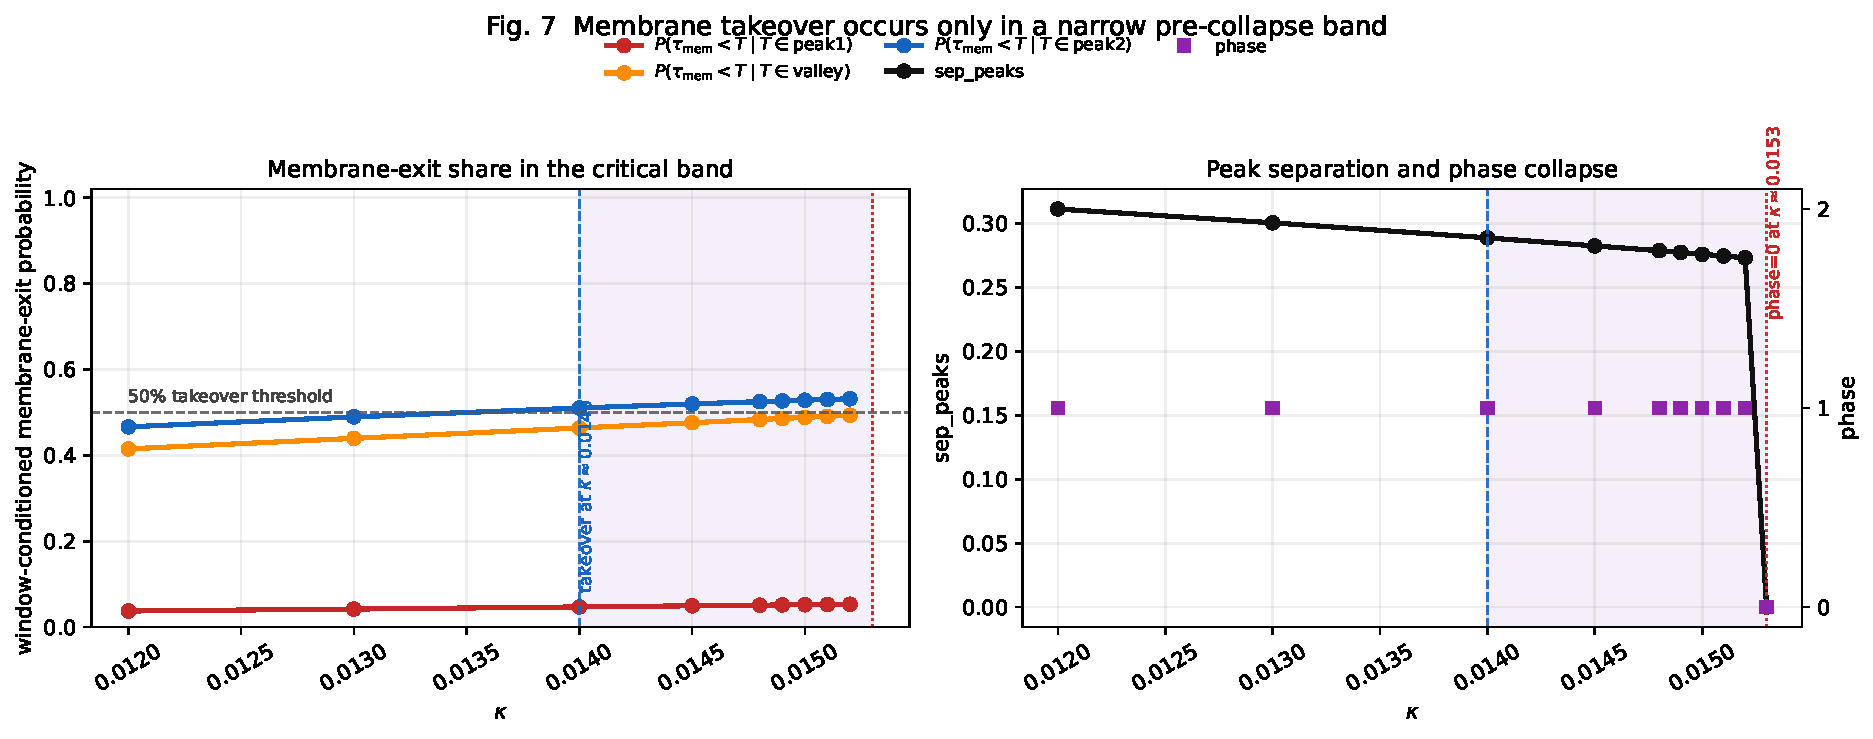
\includegraphics[width=0.98\linewidth]{../artifacts/figures/fig7_takeover_before_collapse.pdf}
  \caption{临界带 probe。左图画的是 `peak1`、`valley`、`peak2` 三窗的 membrane-exit probability；虚线 \(50\%\) 表示 ``membrane-assisted mass 成为多数'' 的接管阈值。右图同时画出 \(\mathrm{sep}_{\mathrm{peaks}}\) 与 phase，用来标出接管与塌缩之间的狭窄窗口。}
  \label{fig:takeover}
\end{figure}

图~\ref{fig:takeover} 给出的信息很直接。

第一，若只看 `peak2`，膜相关质量确实会继续上升，并在
\[
\kappa\approx 0.0140
\]
首次超过 \(50\%\)。此时
\[
P(\tau_{\mathrm{mem}}<T\mid T\in\texttt{peak2})\approx 51.0\%,
\]
说明 ``膜辅助晚峰'' 已经不再只是少数修饰。

第二，这个接管并没有打开一个宽广稳定的 membrane-dominated bimodal 区域。相反，`phase=1` 只维持到
\[
\kappa=0.0152,
\]
而到
\[
\kappa=0.0153
\]
就已经跌成 `phase=0`。与此同时，\(\mathrm{sep}_{\mathrm{peaks}}\) 也从临界带入口的约 \(0.311\) 进一步下降到接近塌缩前的约 \(0.273\)。

第三，这意味着当前参数下真正发生的是：
\begin{quote}
膜相关路径可以在双峰尚未消失时接管第二峰，但这个接管只发生在一个非常窄的 ``塌缩前夕'' 区间，而不是一个宽广稳健的 bimodal 相。
\end{quote}

从机制上说，这进一步支持了前文的结论：在弱到中等通透率里，第二峰主要还是 outside detour / rollback；只有把 \(\kappa\) 推到临界带时，membrane-assisted branch 才会成为多数，但这会立即伴随峰间分离度的持续变差。

\section{临界点本身长什么样}
\begin{figure}[!htbp]
  \centering
  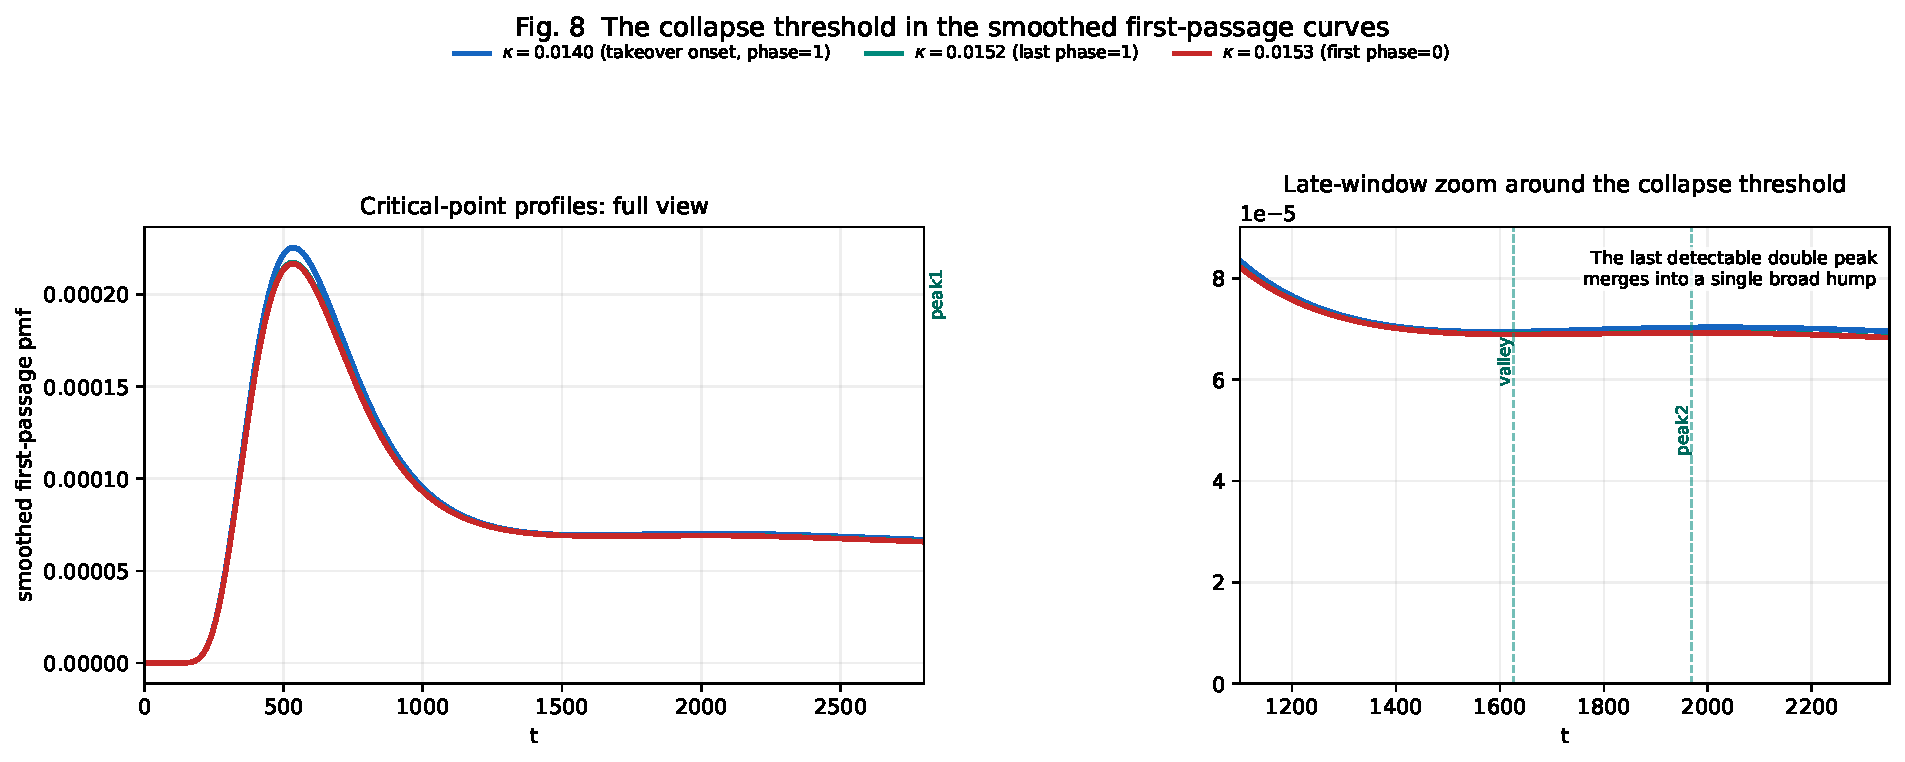
\includegraphics[width=0.98\linewidth]{../artifacts/figures/fig8_critical_collapse_curves.pdf}
  \caption{塌缩临界点附近的 smoothed \(f(t)\) 曲线。这里特意并排放出 \(\kappa=0.0140\)（接管起点）、\(\kappa=0.0152\)（最后一个 `phase=1`）和 \(\kappa=0.0153\)（第一个 `phase=0`）。右图只放大晚峰附近，便于直接看见双峰是如何合并成单个宽 hump 的。}
  \label{fig:critical-curves}
\end{figure}

如果只是想 ``看见临界点''，图~\ref{fig:critical-curves} 就是最直观的答案。

左图说明：从 \(\kappa=0.0140\) 到 \(\kappa=0.0152\)，整体 \(f(t)\) 还保留可检测的双时间尺度结构；但到 \(\kappa=0.0153\) 时，repo-native 判据已经不再把它识别为双峰。

右图更关键。它把晚峰附近单独放大后可以看到：
\begin{itemize}
  \item \(\kappa=0.0152\) 时，仍然还能分辨出 ``第一峰之后再抬起一次'' 的第二个宽峰；
  \item \(\kappa=0.0153\) 时，这个第二峰已经并回成一个更平、更宽的单 hump/shoulder。
\end{itemize}

所以这里的 ``临界点'' 不是某个无限精细数学相变点，而是一个很实用的机制阈值：
\begin{quote}
在 \(\kappa=0.0152\) 还可以说 ``双峰尚存''；到了 \(\kappa=0.0153\)，同一套判据下它就已经塌成单峰形态。
\end{quote}

\section{Fully Reflective Control}
\begin{figure}[!htbp]
  \centering
  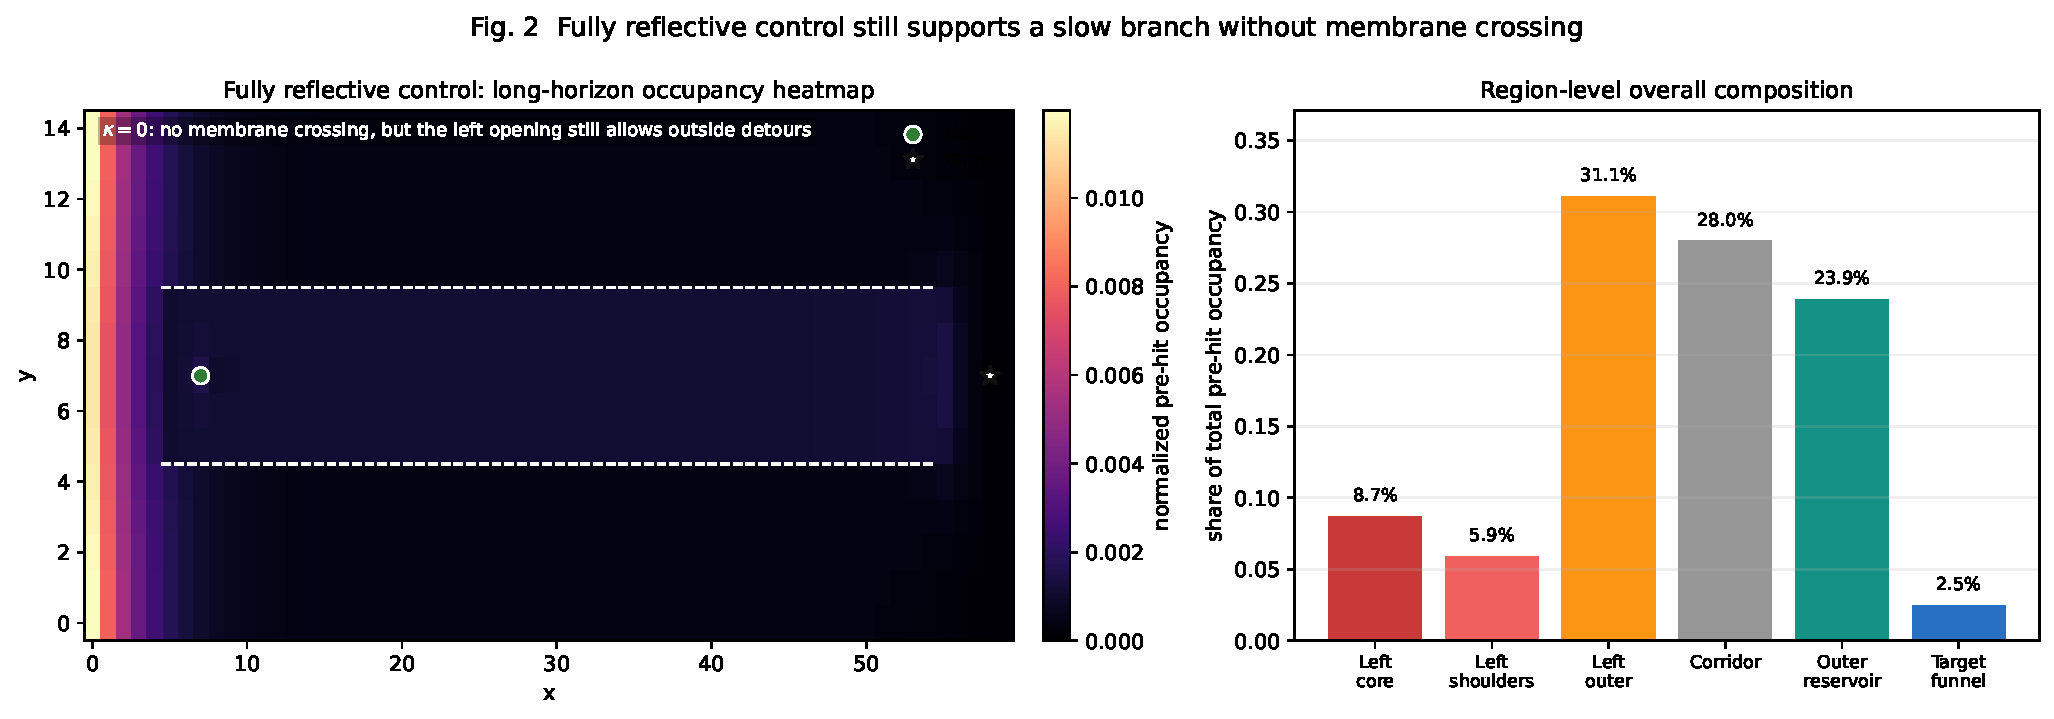
\includegraphics[width=0.98\linewidth]{../artifacts/figures/fig2_fully_reflective_overall_distribution.pdf}
  \caption{fully reflective control \((\kappa=0)\) 的总体 pre-hit occupancy。左图是长时总体热图，右图把总质量按六个机制区汇总。}
  \label{fig:fully-refl}
\end{figure}

图~\ref{fig:fully-refl} 的作用是给出 zero-membrane control。这个 control 下：
\begin{itemize}
  \item \(\tau_{\mathrm{mem}}\) 不可能发生；
  \item 但 `left outer`、`corridor` 和 `outer reservoir` 仍然占据主要质量。
\end{itemize}
具体来说，长时总体 pre-hit occupancy 大约是：
\[
\texttt{left outer}=31.1\%,\quad
\texttt{corridor}=28.0\%,\quad
\texttt{outer reservoir}=23.9\%.
\]
这说明 slow branch 在 \(\kappa=0\) 时已经存在，它来自左端开口允许的绕行/回流，而不是来自膜穿越。

\section{\texorpdfstring{\(\tau_{\mathrm{out}}\)}{tau_out}: 什么时候第一次走出 corridor}
\begin{figure}[!htbp]
  \centering
  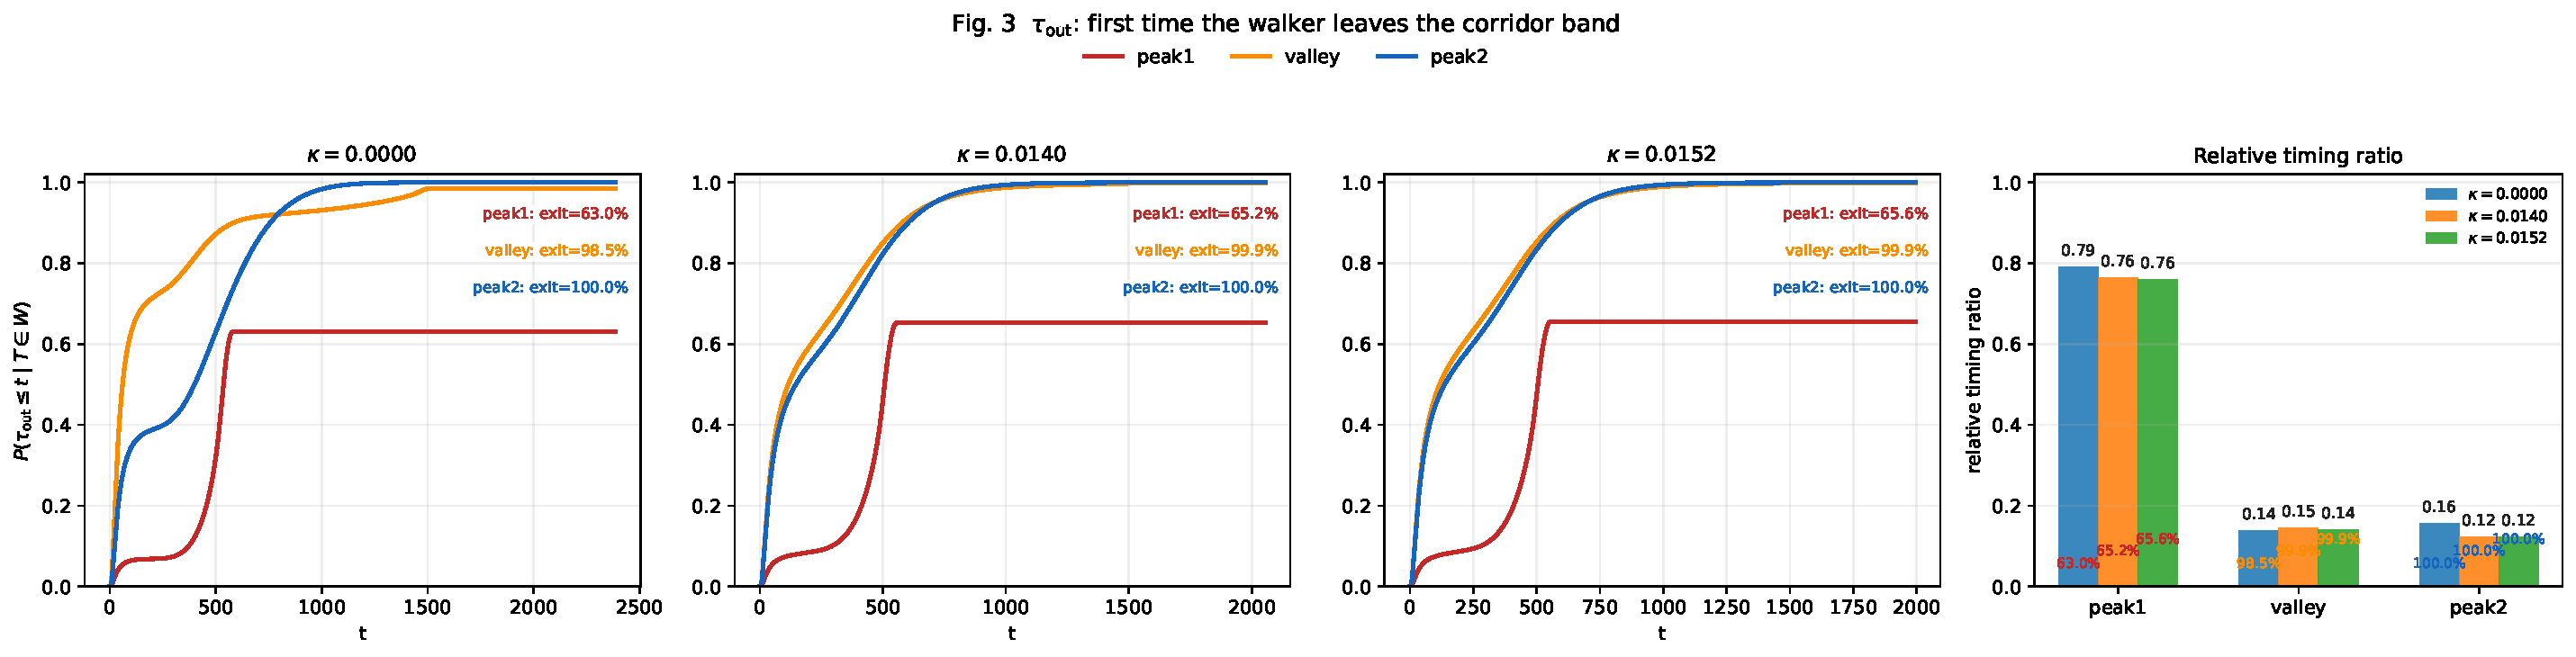
\includegraphics[width=0.98\linewidth]{../artifacts/figures/fig3_tau_out_timing.pdf}
  \caption{\(\tau_{\mathrm{out}}\) 的窗口条件 CDF 与相对 timing ratio。三块 CDF 面板分别对应 \(\kappa=0\)、\(\kappa=0.0140\) 与 \(\kappa=0.0152\)；右图画的是
  \(
  E[\tau_{\mathrm{out}}\mid \tau_{\mathrm{out}}<T,\ T\in W]/E[T\mid T\in W].
  \)}
  \label{fig:tau-out}
\end{figure}

图~\ref{fig:tau-out} 给出的是 ``什么时候离开 corridor''。这里最值得注意的是：
\begin{itemize}
  \item `peak1` 只有约 \(63\%\) 的路径会在命中前离开 corridor；
  \item `valley` 与 `peak2` 基本都是会离开的，概率分别约 \(98.5\%\) 与 \(100\%\)；
  \item 即使推进到 takeover onset 与最后一个 `phase=1`，这些 later-window 的 corridor exits 仍然发生得很早，relative timing ratio 也只有约 \(0.12\sim 0.15\)。
\end{itemize}

这给出一个很清楚的机制解释：later windows 里的路径并不是在末端才偶然离开 corridor，而是通常在自己整条命中轨迹的前段就已经偏出主 corridor 了。换句话说，第二峰更像 ``早早偏出，之后绕行很久''，而不是 ``一路顺着 corridor 走到最后才发生延迟''。

\section{\texorpdfstring{\(\tau_{\mathrm{mem}}\)}{tau_mem}: 什么时候第一次真的穿膜}
\begin{figure}[!htbp]
  \centering
  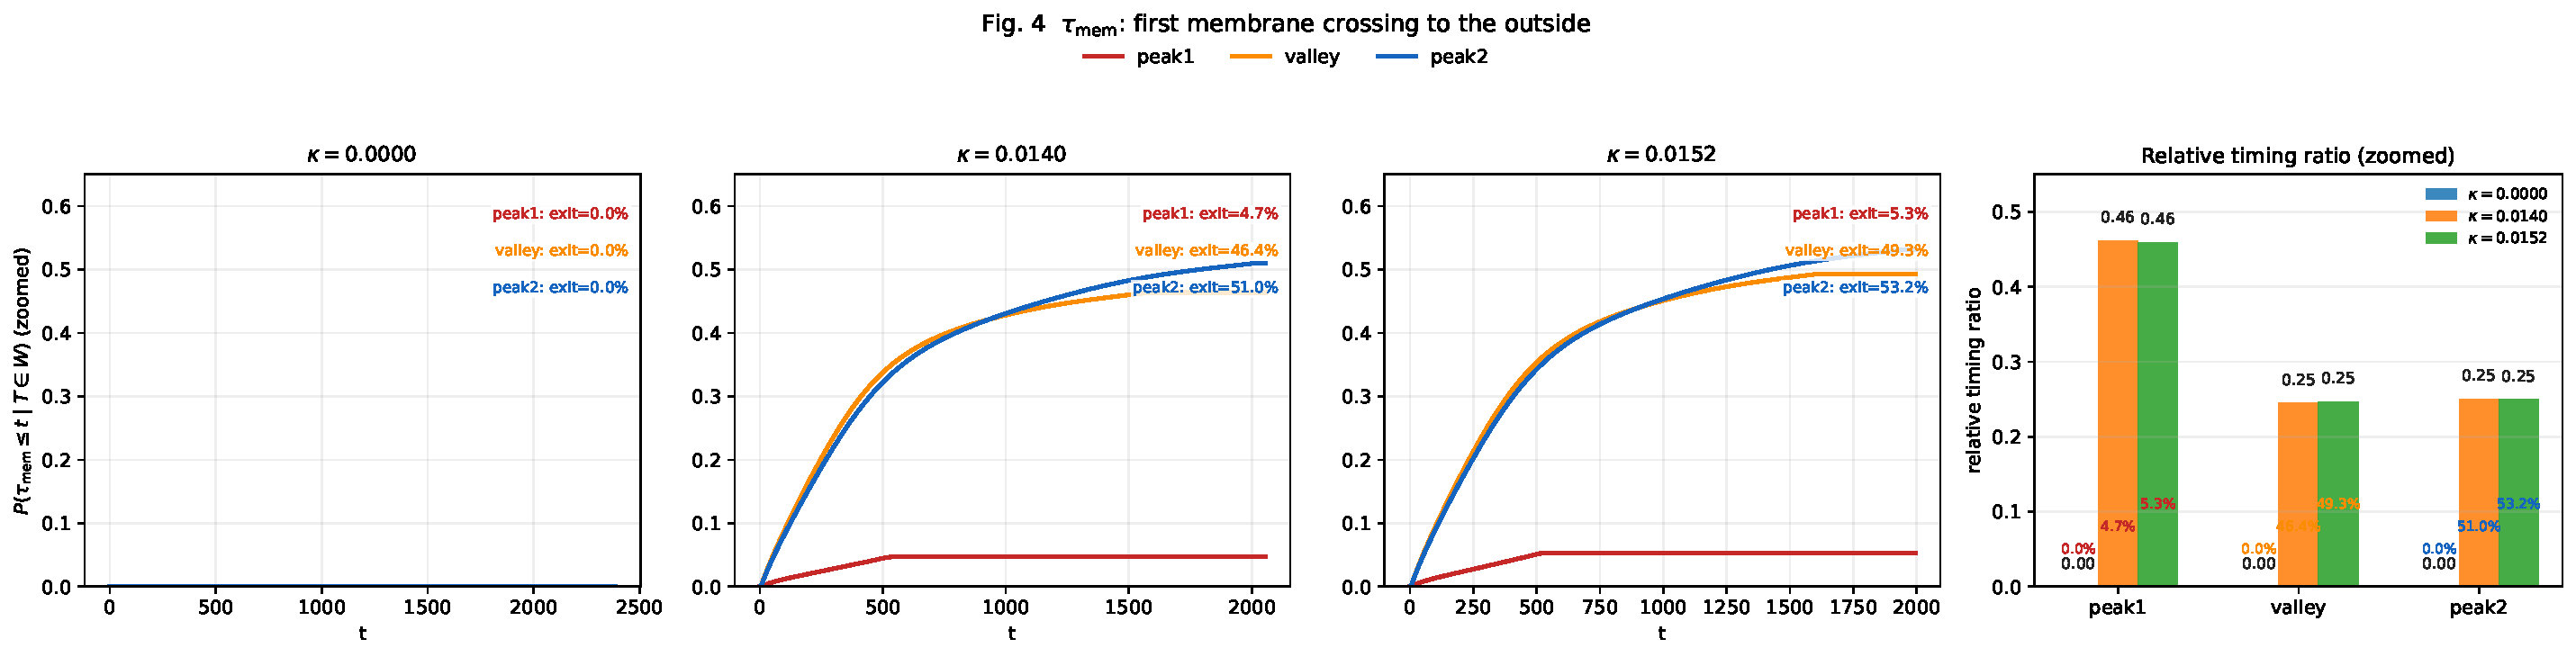
\includegraphics[width=0.98\linewidth]{../artifacts/figures/fig4_tau_mem_timing.pdf}
  \caption{\(\tau_{\mathrm{mem}}\) 的窗口条件 CDF 与相对 timing ratio。左图 \(\kappa=0\) 是严格零控制；中、右图分别展示 takeover onset 的 \(\kappa=0.0140\) 与最后一个 `phase=1` 的 \(\kappa=0.0152\)。为突出膜穿越在临界带内的上升，左侧 CDF 与右侧 ratio 面板都使用了放大的纵轴。}
  \label{fig:tau-mem}
\end{figure}

图~\ref{fig:tau-mem} 把 ``离开 corridor'' 与 ``真正穿膜'' 的差别讲得更直接。

首先，\(\kappa=0\) 时三窗的 membrane-exit probability 都严格是 \(0\)，这验证了 exact helper 的零控制。

其次，直接看两个机制阈值 \(\kappa=0.0140\) 与 \(\kappa=0.0152\)，我们看到：
\[
P(\tau_{\mathrm{mem}}<T\mid T\in\texttt{peak1})\approx 4.68\%\ \text{到}\ 5.31\%,
\]
\[
P(\tau_{\mathrm{mem}}<T\mid T\in\texttt{valley})\approx 46.37\%\ \text{到}\ 49.33\%.
\]
\[
P(\tau_{\mathrm{mem}}<T\mid T\in\texttt{peak2})\approx 51.02\%\ \text{到}\ 53.16\%.
\]
也就是说，在代表性的 critical band 里，later windows 的膜穿越概率已经被推到接管阈值附近甚至略高于 \(50\%\)；这正是为什么 \(\kappa\approx 0.014\) 会成为 ``membrane-assisted mass 开始主导第二峰'' 的 onset。

最后，相对 timing ratio
\[
\frac{E[\tau_{\mathrm{mem}}\mid \tau_{\mathrm{mem}}<T,\ T\in W]}{E[T\mid T\in W]}
\]
在 `valley` 与 `peak2` 中也仍然只有约 \(0.25\)。这说明即使到了 takeover 附近，一旦 later-window 路径真的发生膜穿越，它通常也是在自己命中时间的前段发生，而不是临近吸收时才跨出去。

\section{Early / Late / No-Exit 三分解}
本报告同时给出一个更粗粒度的窗口级 split。对每个窗口 \(W\)，先算 \(E[T\mid T\in W]\)，再用
\[
\tau \le 0.5\,E[T\mid T\in W]
\]
定义 ``early''，其余事件定义为 ``late''。没有发生事件的路径记作 ``no exit''。

\begin{figure}[!htbp]
  \centering
  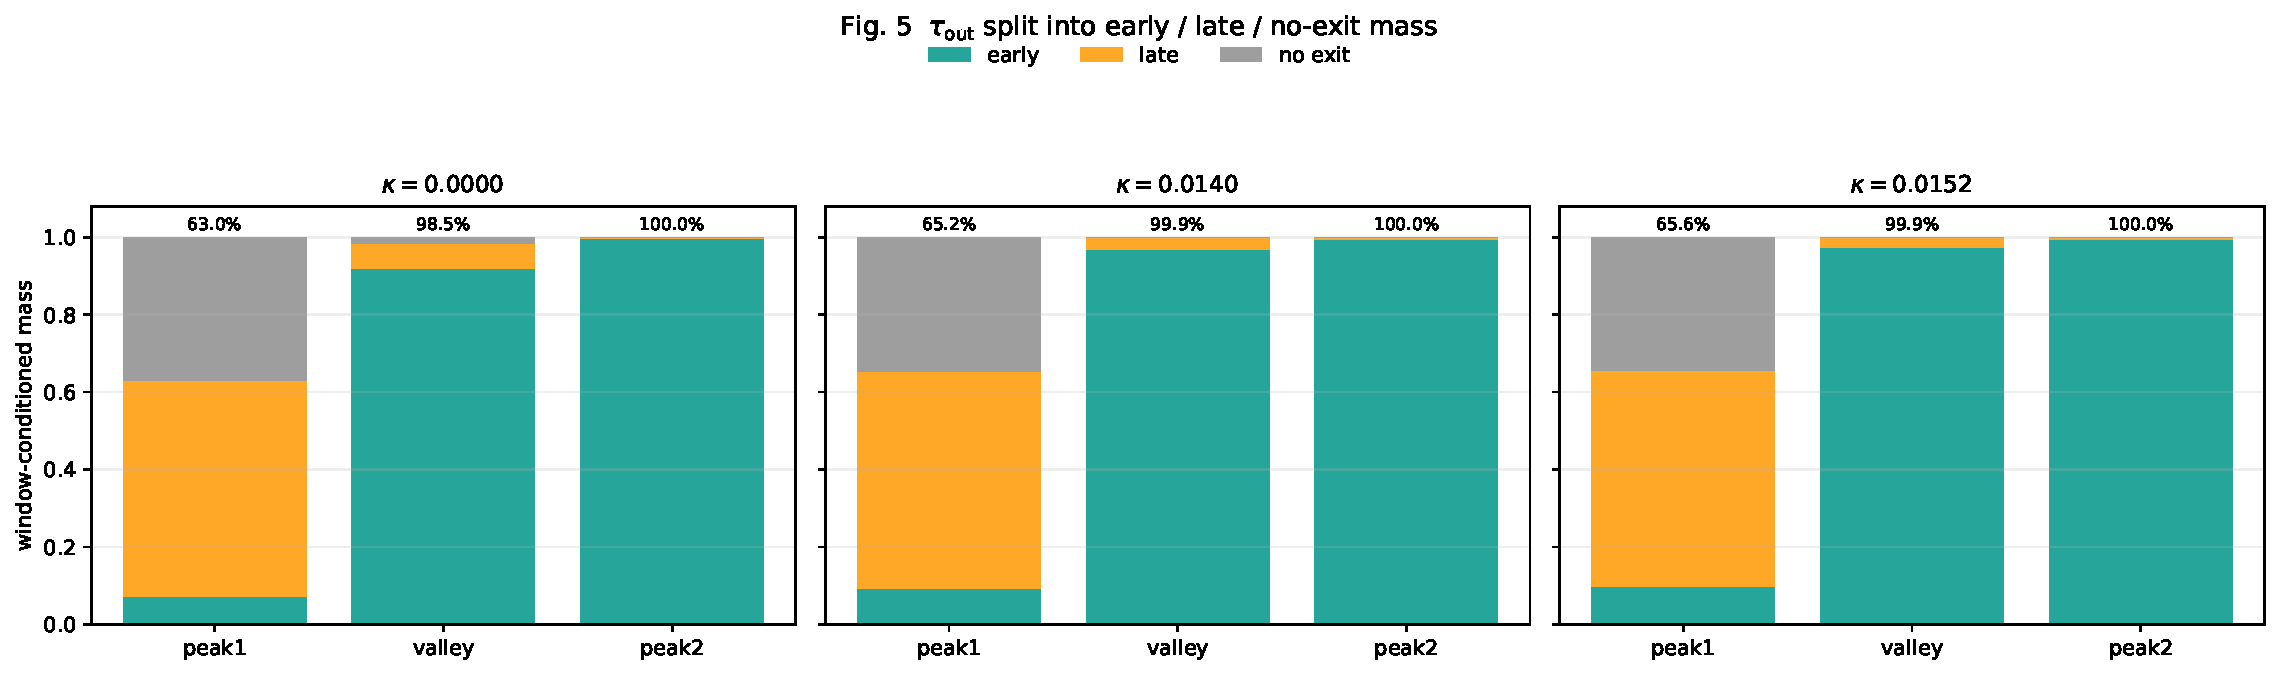
\includegraphics[width=0.98\linewidth]{../artifacts/figures/fig5_tau_out_split.pdf}
  \caption{\(\tau_{\mathrm{out}}\) 的 early / late / no-exit split，展示 \(\kappa=0\)、takeover onset 的 \(\kappa=0.0140\) 与最后一个 `phase=1` 的 \(\kappa=0.0152\)。柱顶数字是总 exit mass。}
  \label{fig:tau-out-split}
\end{figure}

\begin{figure}[!htbp]
  \centering
  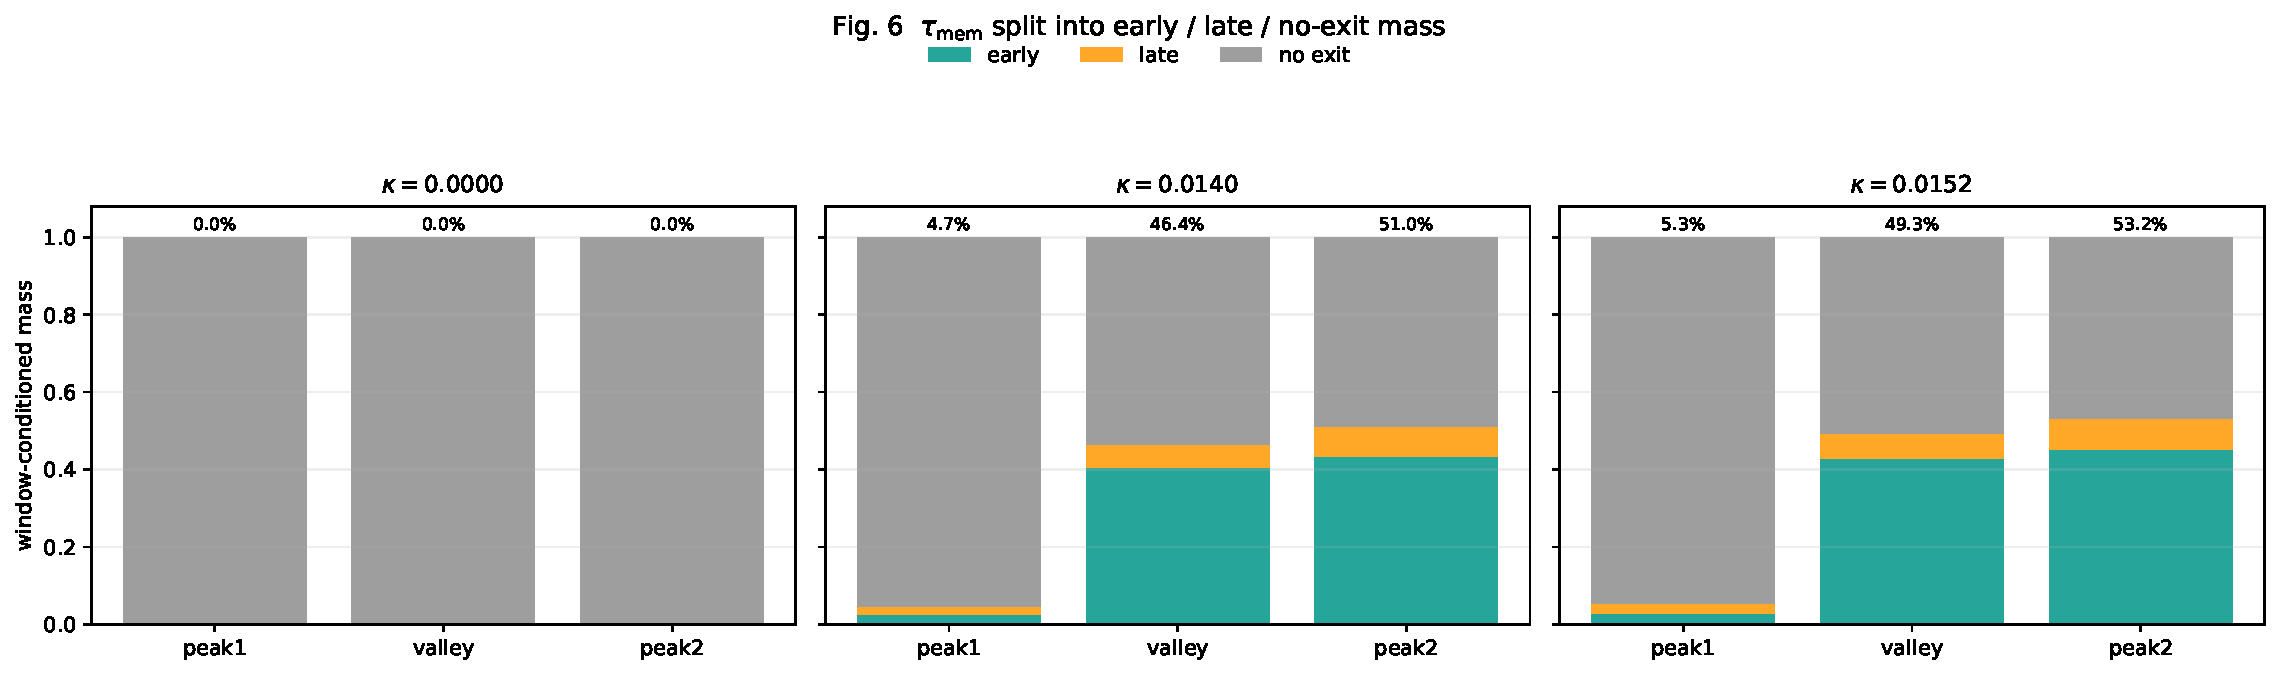
\includegraphics[width=0.98\linewidth]{../artifacts/figures/fig6_tau_mem_split.pdf}
  \caption{\(\tau_{\mathrm{mem}}\) 的 early / late / no-exit split，使用同样三组机制代表值。对于 \(\kappa=0\)，三根柱都应退化成纯 `no exit`。}
  \label{fig:tau-mem-split}
\end{figure}

图~\ref{fig:tau-out-split} 与图~\ref{fig:tau-mem-split} 适合做最直接的机制比对。

对 \(\tau_{\mathrm{out}}\) 而言，`valley` 和 `peak2` 几乎全部都是 early exit，说明这些 later-window 路径的主要特征不是 ``是否出 corridor''，而是 ``出了之后要绕多久才回来''。`peak1` 则不一样，它有显著的 `no exit` mass，而且发生出去的那部分更多落在 late 子块里，这和快通道家族更一致。

对 \(\tau_{\mathrm{mem}}\) 而言，到了 takeover onset 与最后一个 `phase=1`，`valley` 和 `peak2` 的 `no exit` 已经不再占绝对多数；但发生膜穿越的那一部分里，绝大多数仍属于 early exit。于是比较自然的解释是：
\begin{quote}
膜穿越会给 later windows 增加一批更慢的路径，但这批路径在总体晚峰中只占少数，且其穿越动作通常发生在较早阶段。
\end{quote}
图~\ref{fig:takeover} 则补上了下一步：如果继续把 \(\kappa\) 往上推，这批膜相关路径最终的确可以接管 `peak2`；但接管只出现在双峰塌缩前夕，不会形成一个宽广稳定的新相。

\section{代表数值表}
\begin{table}[!htbp]
  \centering
  \footnotesize
  \begin{tabular}{llcccc}
\toprule
$\kappa$ & Observable & peak1 exit & valley exit & peak2 exit & peak2 ratio \\
\midrule
0.0000 & $\tau_{\mathrm{out}}$ & 63.0\% & 98.5\% & 100.0\% & 0.16 \\
0.0000 & $\tau_{\mathrm{mem}}$ & 0.0\% & 0.0\% & 0.0\% & 0.00 \\
0.0140 & $\tau_{\mathrm{out}}$ & 65.2\% & 99.9\% & 100.0\% & 0.12 \\
0.0140 & $\tau_{\mathrm{mem}}$ & 4.7\% & 46.4\% & 51.0\% & 0.25 \\
0.0152 & $\tau_{\mathrm{out}}$ & 65.6\% & 99.9\% & 100.0\% & 0.12 \\
0.0152 & $\tau_{\mathrm{mem}}$ & 5.3\% & 49.3\% & 53.2\% & 0.25 \\
\bottomrule
\end{tabular}

  \caption{代表性 \(\kappa\) 下两个 observable 的窗口条件 exit probability 与 `peak2` relative timing ratio。}
  \label{tab:rep}
\end{table}

表~\ref{tab:rep} 把最常用的数值压成一眼能看的形式。若只记住一组数，建议记：
\begin{itemize}
  \item \(\kappa=0\) 时，\(\tau_{\mathrm{mem}}\) 三窗全为 \(0\)，但 \(\tau_{\mathrm{out}}\) 在 `valley/peak2` 已经是 \(98.5\%\) 与 \(100\%\)；
  \item \(\kappa=0.006\) 时，`peak2` 的 \(\tau_{\mathrm{mem}}\) 也只有约 \(27.9\%\)，仍明显小于 `peak2` 的 \(\tau_{\mathrm{out}}\approx 100\%\)。
\end{itemize}
这组对照几乎已经把 ``第二峰主要来自哪里'' 这个问题回答完了：它主要来自离开 corridor 后的 detour/rollback，而不是来自膜穿越本身。

\section*{总结}
从 fully reflective 到 weakly permeable 的整个 continuation 看下来，这个 one-target 双峰最稳的机制图景是：
\begin{enumerate}
  \item 第一峰主要对应直接 corridor transport；
  \item 第二峰在 \(\kappa=0\) 时就已经存在，说明 baseline slow branch 来自左端开口允许的 outside detour；
  \item 对称半透膜会逐步增加 later windows 的 membrane-assisted branch；到 \(\kappa=0.006\) 时它已经清晰可见，但在当前参数下仍是一层次级修饰；
  \item 若继续把 \(\kappa\) 推到临界带，`peak2` 的 membrane-assisted mass 会在 \(\kappa\approx 0.014\) 左右超过 \(50\%\)；但这种接管只维持到塌缩前夕，因为 \(\kappa=0.0153\) 时双峰已不再被检测到；
  \item 因而若要理解 ``谁贡献第二峰''，优先看 \(\tau_{\mathrm{out}}\)；若要分辨 ``膜到底加了多少''，再看 \(\tau_{\mathrm{mem}}\)。
\end{enumerate}

\end{document}
